\documentclass[tikz,border=6pt]{standalone}
\usetikzlibrary{arrows.meta,positioning}
\begin{document}
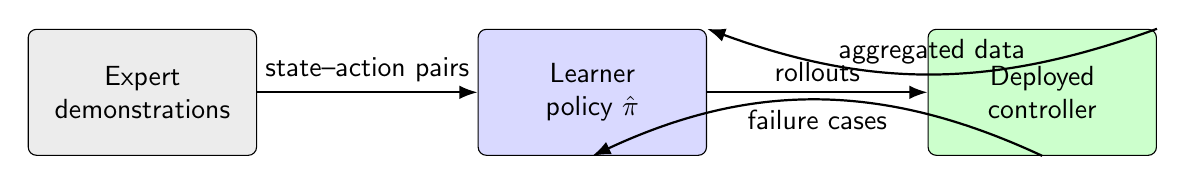
\begin{tikzpicture}[font=\sffamily,node distance=2.8cm,>=Latex]
  \tikzstyle{stage}=[draw,rounded corners=3pt,minimum width=2.9cm,minimum height=1.6cm,align=center]
  \node[stage,fill=gray!15] (expert) {Expert\\demonstrations};
  \node[stage,fill=blue!15,right=of expert] (learner) {Learner\\policy $\hat{\pi}$};
  \node[stage,fill=green!20,right=of learner] (policy) {Deployed\\controller};
  \draw[->,thick] (expert) -- node[above]{state--action pairs} (learner);
  \draw[->,thick] (learner) -- node[above]{rollouts} (policy);
  \draw[->,thick,bend left=20] (policy.north east) to node[above]{aggregated data} (learner.north east);
  \draw[->,thick,bend right=25] (policy.south) to node[below]{failure cases} (learner.south);
\end{tikzpicture}
\end{document}
